\documentclass[10pt,aspectratio=169]{beamer}

% All the boilerplate is in deslides.sty
\usepackage{deslides}

\author{Ji\v{r}\'i Lebl}

\institute[OSU]{%
Oklahoma State University%
%Departemento pri Matematiko de Oklahoma {\^S}tata Universitato%
}

\title{4. Slope fields (Notes on Diffy Qs, 1.2)}

\date{}

\begin{document}

\begin{frame}
\titlepage

%\bigskip

\begin{center}
The textbook: \url{https://www.jirka.org/diffyqs/}
\end{center}
\end{frame}

\begin{frame}
Consider the general first order equation \quad $y' = f(x,y)$.

\medskip
\pause

We can't always solve such an equation explicitly,

\pause
but we can always figure out the shape and behavior of the solutions.

\medskip
\pause

At each $(x,y)$ in the plane, the solution would have a slope $y' = f(x,y)$.

\medskip
\pause

So why not draw a little line with the slope $f(x,y)$ at the point $(x,y)$.
\pause
And do it for all $(x,y)$.

\medskip

E.g., $y'=xy$. \pause

At $(2,1.5)$, draw a line of slope
$xy = 2 \times 1.5 = 3$

\vspace*{-24pt}
\hspace*{3in}\visible<7>{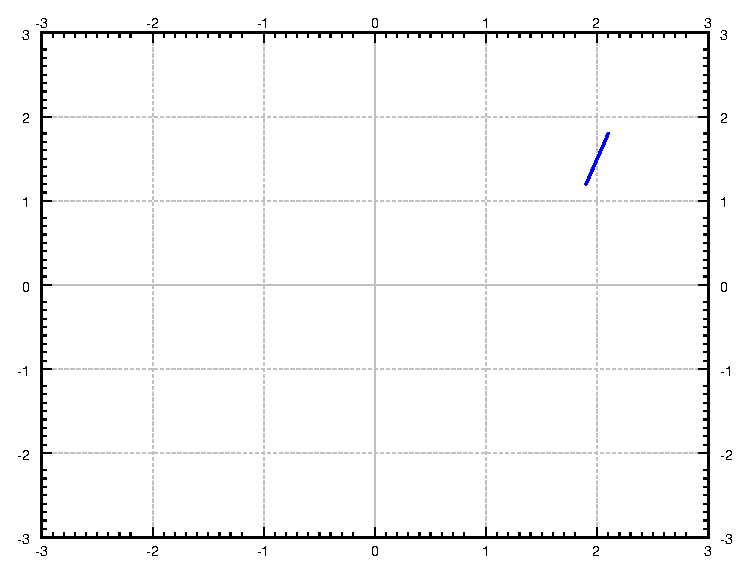
\includegraphics[width=2.5in]{../figures/1-3-xysl-one}}

\vspace*{-1.53in}
\pause
Now do it for a grid of points.

\vspace*{-42pt}
\hspace*{3in}\visible<8-10>{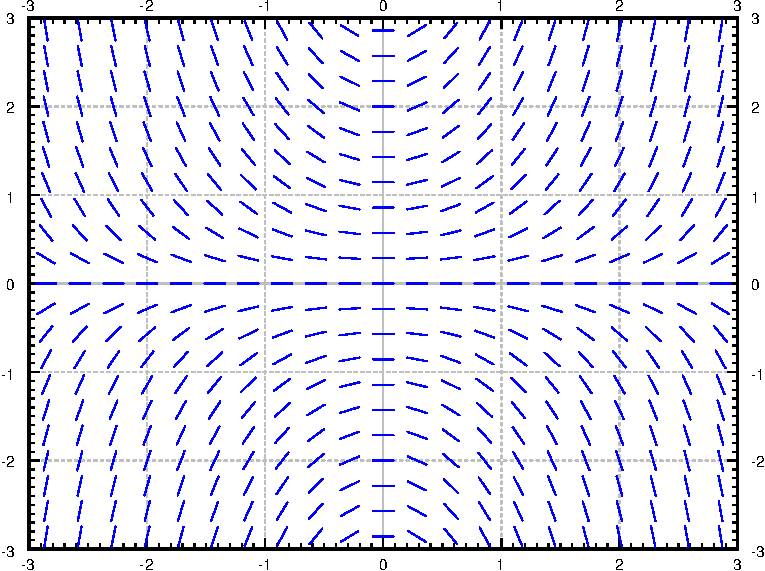
\includegraphics[width=2.5in]{../figures/1-3-xysl}}

\vspace*{-1.3in}
\pause

This is called the \emph{slope field}.

\pause
\medskip

Given a specific initial condition,

$y(x_0)=y_0$, we could draw a solution.

\pause
\medskip

E.g., $y(0) = 0.2$, $y(0) = 0$, and $y(0) = -0.2$.

\vspace*{-107pt}
\hspace*{3in}\visible<11->{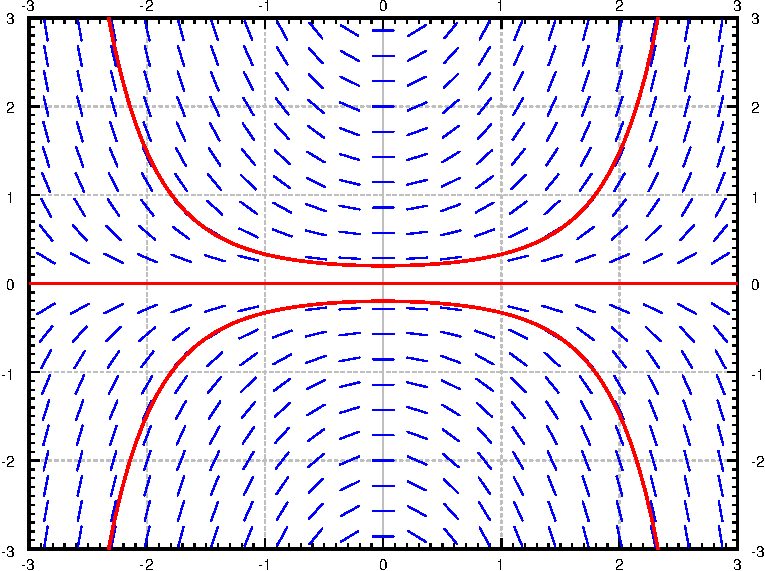
\includegraphics[width=2.5in]{../figures/1-3-xysl-sol}}

\pause
\vspace*{-0.33in}

We can tell just by the slope field that $y(0) > 0$

leads to very different behavior from $y(0) < 0$.

\end{frame}

\begin{frame}

Here's another example: $y'=-y$ with a few solutions given:

\begin{center}
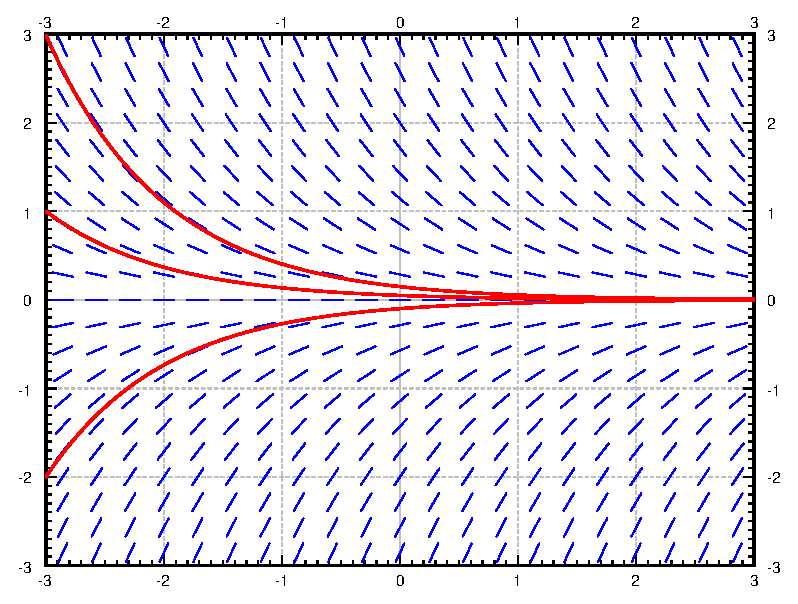
\includegraphics[width=3in]{../figures/1-3-mysl-sol}
\end{center}

\pause

Note how in this case we can tell from the slope field
that all solutions just tend to $y=0$.
\end{frame}

\begin{frame}
Given a problem
\begin{equation*}
y' = f(x,y), \qquad y(x_0) = y_0.
\end{equation*}
\begin{enumerate}[(i)]
\item\pause Does a solution \emph{exist}?
\item\pause Is the solution \emph{unique} (if it exists)?
\end{enumerate}

\medskip
\pause

The answer is usually yes to both.

\pause
If the answer is no, you probably do not have the right model.

\medskip
\pause

\textbf{Example:}
Answer to (i) can be no:

\quad $y' = \frac{1}{x}, \qquad y(0) = 0$.

\pause (or the more harmless
looking $x y' = 1$)

\medskip
\pause

Integration yields: $y = \ln \, \lvert x \rvert + C$. \quad

\pause
There is no solution at $x=0$.

\vspace*{-68pt}
\hspace*{3in}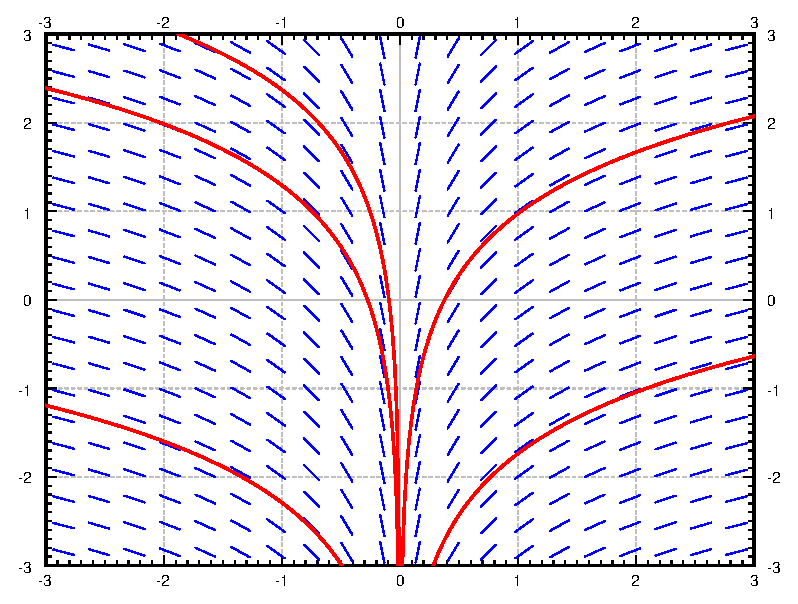
\includegraphics[width=2.5in]{../figures/1-3-xinv-sol}

\end{frame}

\begin{frame}
\textbf{Example:}
\begin{equation*}
y' = 2 \sqrt{\lvert y \rvert}, \qquad y(0) = 0 .
\end{equation*}
\pause
Note that $y=0$ is a solution.
\pause
But another solution is the function
\begin{equation*}
y(x) =
\begin{cases}
x^2 & \text{if } \; x \geq 0,\\
-x^2 & \text{if } \; x < 0.
\end{cases}
\end{equation*}

\begin{center}
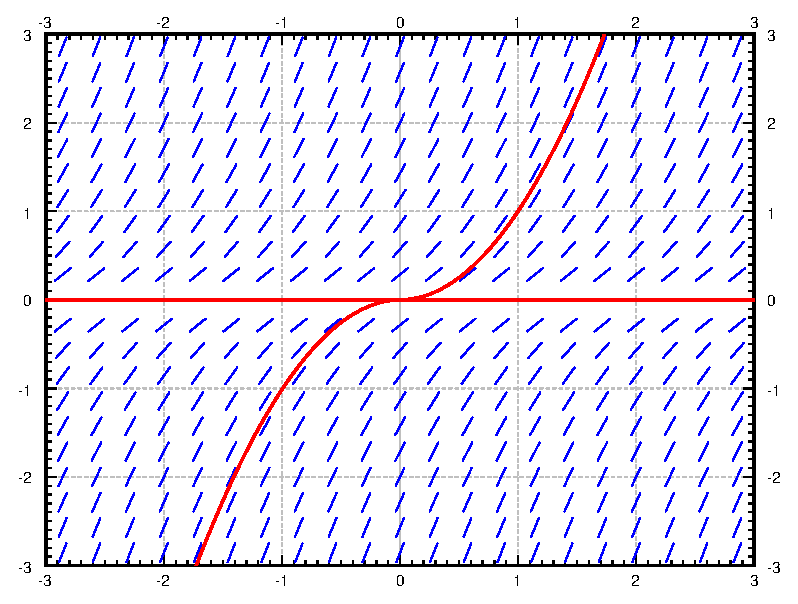
\includegraphics[width=2.5in]{../figures/1-3-sqrt-sol}
\end{center}

So answer to (ii) can also be false.
\end{frame}

\begin{frame}
All hope is not lost!

\pause

\begin{theorem}[Picard's theorem on existence and uniqueness]%
If $f(x,y)$ is continuous and $\frac{\partial f}{\partial y}$ exists and is
continuous near $(x_0,y_0)$, then a solution to
\begin{equation*}
y' = f(x,y), \qquad y(x_0) = y_0,
\end{equation*}
exists (for $x$ in some interval) and is unique.
\end{theorem}

\pause

E.g., \quad $y' = \nicefrac{1}{x}$, $y(0) = 0$
\quad and \quad $y' = 2 \sqrt{\lvert y \rvert}$, $y(0) = 0$ \quad
do not satisfy the hypotheses.

\medskip
\pause

\textbf{Example:}
Remember
\quad
$
y' = y^2, \qquad y(0) = A$ \quad ?

\medskip
\pause

If $A=0$, then $y=0$ is the solution.  It exists for all $x$.

\medskip
\pause

If $A\not=0$, then solution is $y=\frac{1}{C-x}$.

\medskip
\pause

$A = y(0) = \frac{1}{C-0} = \nicefrac{1}{C}$
\pause
\wthus
$C=\nicefrac{1}{A}$
\pause
\wthus
The solution is
$\displaystyle
y = \frac{1}{\nicefrac{1}{A} - x}$.

\medskip
\pause

If $A=1$, the solution blows up when $x=1$.
The solution exists for $x < 1$.

\medskip
\pause

If $A=100$, the solution blows up when $x=\frac{1}{100}=0.01$.
The solution exists for $x < 0.01$.
\end{frame}

\end{document}
